\documentclass{article}

% Paquetes plantilla
\usepackage[square, numbers, sort]{natbib}
% \usepackage{cite}
\usepackage{graphicx}
\usepackage[utf8]{inputenc}
\usepackage{amsmath,amssymb,amsfonts}
\usepackage{algorithmic}
\usepackage{textcomp}
\usepackage{subfig}
\usepackage{float}
\usepackage{empheq}
\usepackage{mathtools}
\usepackage[spanish]{babel}
\usepackage[paper=a4paper,margin=2.75cm]{geometry}
\usepackage{booktabs} % for tables
\usepackage[colorlinks = true,
            linkcolor = blue,
            urlcolor  = blue,
            citecolor = orange,
            anchorcolor = blue]{hyperref} % for hyperlinks
\usepackage{xcolor} % text colors
% Paquetes extra
\usepackage{subcaption, booktabs, siunitx, tikz}
\usepackage{pgfplots}
\pgfplotsset{compat=1.15}
\usepackage{mathrsfs}
\usetikzlibrary{arrows}
\tikzset{every picture/.style={line width=0.75pt}} %set default line width to 0.75pt 

\sisetup{
    round-mode          = places, % Rounds numbers
    round-precision     = 2, % to 2 places
}

\usepackage{titlesec}

\setcounter{secnumdepth}{4}

\titleformat{\paragraph}
{\normalfont\normalsize\bfseries}{\theparagraph}{1em}{}
\titlespacing*{\paragraph}
{0pt}{3.25ex plus 1ex minus .2ex}{1.5ex plus .2ex}

% Directorio con imagenes
\graphicspath{{./figs/}}

% Cabecera del documento
% ======================================================================

% Titulo
\title{PROYECTO INTEGRADOR AUTÓMATAS Y CONTROL DISCRETO}

% Autores
\author{Juan Pablo Sibecas \\ juan.sibecas@gmail.com \\Matias Gaviño\\ matias.linares.g@gmail.com \\ Autómatas y Control Discreto, Facultad de Ingeniería, \\ Universidad Nacional de Cuyo, \\ Mendoza, Argentina}

% Fecha
\date{Junio de 2024}

% Cuerpo del documento
% ======================================================================
\begin{document}

% Comandos definidos por el autor
\renewcommand{\tablename}{Tabla}
% \renewcommand{\color{blue}{#1}}{\azul}

% Crear cabecera
\maketitle

% Resumen
% ======================================================================
\begin{abstract}\label{sec:abstract}

\end{abstract}

\newpage

\section{Introducción} \label{sec:intro}


El presente informe aborda el control de una grúa portuaria destinada a la carga, descarga y reubicación de contenedores entre el barco y las bahías de carga. El objetivo es mejorar la eficiencia del sistema mediante trayectorias de movimiento que sean tanto suaves como rápidas.

Para desarrollar este control, se comienza con el modelado del sistema físico, que consta de un carro para el movimiento horizontal y un sistema de izaje para el movimiento vertical. Ambos movimientos están acoplados por la carga, la cual consiste en un contenedor y un "spreader" que lo sostiene. La traslación y el izaje son accionados por motores eléctricos, lo que permite un control preciso de las trayectorias.

El desarrollo del informe incluye el modelado del sistema físico, obteniendo las ecuaciones de movimiento y utilizando Simulink para simular su comportamiento. A continuación, se diseña un control híbrido de tres niveles: el nivel 2 se encarga del control en tiempo discretizado para los motores que accionan el izaje y el carro; el nivel 1 consiste en un controlador discreto basado en eventos, que genera trayectorias suaves y eficientes; y el nivel 0 actúa como sistema de seguridad, asegurando que el sistema entre en un estado seguro en caso de fallas. Para la simulación del controlador, se emplea el software Matlab/Simulink, y luego se implementa en Codesys para simular su ejecución en un PLC.


\section{Desarrollo} \label{sec:desarrollo}
    \subsection{Modelo del Sistema Físico} \label{sec:plantModel}

        El modelo del sistema se simplifica a un control de posición de la carga en el plano. No se tendran en cuenta grados liberdad que no estan complendidos en el plano perpendicular el eje longitudinal del muelle. Se considera que la esturcuruta de la grua es rigida y que no se producen vibraciones, no así los cable que se consideran flexibles.
        Para el desarrollo de las ecuaciones se parde desde lo desarrollado en el enunciado del trabajo practico.
        
        \subsubsection{Subsistema de Izaje}
            Segunda ley de Newton del lado tambor:
            \begin{equation} \label{eq:tamborIzaje}
                J_{hd+hEb} \frac{d \omega_{hd}}{dt} = T_{hd}(t) + T_{hEb}(t) - b_{hd} \omega_{hd}(t) - T_{hdl}(t)
            \end{equation}

            Segunda ley de Newton del lado motor:
            \begin{equation} \label{eq:motorIzaje}
                J_{hm+hb} \frac{d \omega_{hm}}{dt} = T_{hm}(t) + T_{hb}(t) - b_{hm} \omega_{hm}(t) - T_{hml}(t)
            \end{equation}

            relacion de transmision
            \begin{equation} \label{eq:transmisionIzaje}
                i_h = \frac{\omega_{hm}(t)}{\omega_{hd}(t)} = \frac{T_{hd}(t)}{T_{hml}(t)}
            \end{equation}

            si reemplazo \ref{eq:transmisionIzaje} en \ref{eq:motorIzaje} y despejo $T_{hd}(t)$

            \begin{equation} \label{eq:Thd}
                T_{hd}(t) = J_{hm+hb} \frac{d \omega_{hd}}{dt} {i_h}^2 - b_{hm} \omega_{hd}(t) {i_h}^2 + i_h (T_{hm}(t) + T_{hb}(t))
            \end{equation}

            reemplazando en \ref{eq:tamborIzaje} y operando se obtiene

            \begin{equation} \label{eq:izajeThdl}
                (J_{hd+hEb} + J_{hm+hb} i_h^2) \frac{d \omega_{hd}}{dt} = - (b_{hd} + b_{hm}i_h^2) \omega_{hd}(t) + i_h (T_{hm}(t) + T_{hb}(t)) + T_{hEb}(t) - T_{hdl}(t)
            \end{equation}

            como $T_{hdl}(t) = F_{hw}(t)*r_{hd}$, $2V_h = r_{hd}*\omega_{hd}(t)$ y $V_h = -\frac{dl_h(t)}{dt}$ y dividiendo por $r_{hd}$:

            \begin{equation} \label{eq:izajeFhw}
                2\frac{(J_{hd+hEb} + J_{hm+hb} i_h^2)}{r_{hd}^2} \frac{d^2 l_h(t)}{dt^2} = - 2\frac{(b_{hd} + b_{hm}i_h^2)}{r_{hd}^2} \frac{d l_h(t)}{dt} - \frac{i_h}{r_{hd}} (T_{hm}(t) + T_{hb}(t)) - \frac{T_{hEb}(t)}{r_{hd}} + F_{hw}(t)
            \end{equation}
            
            Reemplazando por parametros equivalentes:
            
            \begin{equation} \label{eq:izajeEquiv}
                M_{Eh} \ddot{l_h}(t) = - b_{Eh} \dot{l_h}(t) - \frac{i_h}{r_{hd}} (T_{hm}(t) + T_{hb}(t)) - \frac{T_{hEb}(t)}{r_{hd}} + F_{hw}(t)
            \end{equation}

            Donde

            \begin{align} \label{eq:izajeParamsEquiv}
                M_{Eh} = 2\frac{(J_{hd+hEb} + J_{hm+hb} i_h^2)}{r_{hd}^2}\\
                b_{Eh} = 2\frac{(b_{hd} + b_{hm}i_h^2)}{r_{hd}^2}\\
            \end{align}

            En la figura \ref{fig:hoisting_drive_simulink} se muestra el modelo de Simulink del subsistema de izaje. Se observa que se implenta la ecuación \ref{eq:izajeEquiv} con sus respectivos parámetros equivalentes. Además, se incluye el modelo del sistema de freno y freno de emergencia. 

            \begin{figure} [H]
                \centering
                \includegraphics[width=1\textwidth]{figs/hoisting_drive_simulink.png}
                \caption{Modelo de Simulink del subsistema de izaje}
                \label{fig:hoisting_drive_simulink}
            \end{figure}

            \textbf{Modelo del cable de izaje}

            \begin{figure} [H]
                \centering
                \includegraphics[width=1\textwidth]{figs/hoisting_cable_mode_simulink.png}
                \caption{Modelo de Simulink del cable de izaje}
                \label{fig:hoisting_cable_mode_simulink}
            \end{figure}

            

        \subsubsection{Subsistema Carro}
            Segunda ley de Newton del lado tambor:
            \begin{equation} \label{eq:tamborCarro}
                J_{td} \frac{d \omega_{td}(t)}{dt} = T_{td}(t) - b_{td} \omega_{td}(t) - T_{tdl}(t)
            \end{equation}

            Segunda ley de Newton del lado motor:
            \begin{equation} \label{eq:motorCarro}
                J_{tm+tb} \frac{d \omega_{tm}(t)}{dt} = T_{tm}(t) + T_{tb}(t) - b_{tm} \omega_{tm}(t) - T_{tml}(t)
            \end{equation}

            relacion de transmision
            \begin{equation} \label{eq:transmisionCarro}
                i_t = \frac{\omega_{tm}(t)}{\omega_{td}(t)} = \frac{T_{td}(t)}{T_{tml}(t)}
            \end{equation}

            si reemplazo \ref{eq:transmisionCarro} en \ref{eq:motorCarro} y despejo $T_{td}(t)$

            \begin{equation} \label{eq:Ttd}
                T_{td}(t) = J_{tm+tb} \frac{d \omega_{td}(t)}{dt} {i_t}^2 - b_{tm} \omega_{td}(t) {i_t}^2 + i_t (T_{tm}(t) + T_{tb}(t))
            \end{equation}

            Reemplazo \ref{eq:Ttd} en \ref{eq:tamborCarro} y reordeno:

            \begin{equation} \label{eq:carroTtdl}
                (J_{td} + J_{tm+tb}*i_t^2) \frac{d \omega_{td}(t)}{dt} = i_t (T_{tm}(t) + T_{tb}(t)) - (b_{td} + b_{tm}{i_t}^2) \omega_{td}(t) - T_{tdl}(t)
            \end{equation}
        
            Como $\omega_{td}(t) r_{td} = V_{td}(t)$, $F_{tw}(t)r_{td} = T_{tdl}(t)$ y $V_{td}(t) = \frac{d x_{td}}{dt}$ y dividiendo por $r_{td}$:
            
            \begin{equation} \label{eq:carroFtw}
                \frac{(J_{td} + J_{tm+tb}*i_t^2)}{r_{td}^2} \frac{d^2 x_{td}(t)}{dt^2} = - \frac{(b_{td} + b_{tm}{i_t}^2)}{r_{td}^2} \frac{d x_{td}(t)}{dt} + \frac{i_t}{r_{td}} (T_{tm}(t) + T_{tb}(t)) - F_{tw}(t)
            \end{equation}

            Reemplazando por parametros equivalentes se obtiene la ecuacion del tambor del subsistema carro:

            \begin{equation} \label{eq:TamborCarro}
                M_{Etd} \ddot{x_{td}}(t) = - b_{Etd} \dot{x_{td}}(t) + \frac{i_t}{r_{td}} (T_{tm}(t) + T_{tb}(t)) - F_{tw}(t)
            \end{equation}

            La ecuacion de movimiento del carro es:

            \begin{equation} \label{eq:Carro}
                M_t \ddot{x_{t}}(t) = - b_t \dot{x_{t}}(t) + F_{tw}(t) + 2F_{hw}(t)\sin{\theta_l(t)}
            \end{equation}

            Y la fuerza transmitida por el cable del subsistema carro es:

            \begin{equation} \label{eq:fuerzaCableCarro}
                F_{tw}(t) = K_{tw}(x_{td}(t) - x_t(t)) + b_{tw}(\dot{x_{td}}(t) - \dot{x_t}(t))
            \end{equation}

            \begin{figure}
                \centering
                \includegraphics[width=1\textwidth]{figs/trolley_drive_simulink.png}
                \caption{Modelo de Simulink del subsistema carro}
                \label{fig:carriage_drive_simulink}
            \end{figure}

                
        \subsection{Diseño del controlador}

            \begin{equation}\label{eq:PID}
                T_m'(t) = b_ae_\omega(t) + K_{sa} e_\theta(t) + K_{sia}\int e_\theta(t) dt
            \end{equation}
            Por lo tanto, por Laplace:
            \begin{equation}\label{eq:PID_Laplace}
                T_m(s) = G(s)[b_aE_\omega(s) + K_{sa} \frac{1}{s} + K_{sia} \frac{1}{s^2}]E_\theta(s)
            \end{equation}

            Donde \(G_T(s)\) es la función de transferencia del modulador de torque que, como se supone ideal, es igual a 1.


            Para obtener la expresión que nos permita obtener las constante que definen al controlador se remplaza la ecuacion \ref{eq:PID} en la ecuacion de movimiento del izaje y del carro, se obtiene:
            Para el izaje, reemplazando \ref{eq:PID} en \ref{eq:izajeEquiv} y transformandola con Laplace, se obtiene:
            \begin{equation}\label{eq:izajeControl}
                M_{Eh} \ddot{L_h}(s) = - b_{Eh} sL_h(s) - \frac{i_h}{r_{hd}} [G(s)[b_aE_\omega(s) + K_{sa} \frac{1}{s} + K_{sia} \frac{1}{s^2}]E_\theta(s)] + F_{hw}(s)
            \end{equation}
            despejando 


        \subsubsection{Control del Carro}

            Segun el modelo del sistema, la ecuacion de movimiento del carro es:
            \begin{equation}
                M_t \ddot{x_{t}}(t) = - b_E \dot{x_{t}}(t) + \frac{i_t}{r_{td}} T_{tm}(t) - F_{L}(t) 
            \end{equation}

            Se desacopla el primer termino sustituyendo:
            \begin{equation}
            T_m(t) = T_{tm}^*(t) + \frac{r_{td} b_E}{i_t} \dot{x_t}(t)
            \end{equation}

            Además, si no se tiene en cuenta \(F_{L}(t)\) se obtiene:
            \begin{equation}
                M_E \ddot{x_{t}}(t) =  \frac{i_t}{r_{td}} T_{tm}^*(t) 
            \end{equation}

            Aplicando la transformada de Laplace y definiendo como ley de control un controlador PID, se obtiene:

            \begin{equation}
                M_E s^2 X_t(s) =  \frac{i_t}{r_{td}} T_{tm}^*(s)
            \end{equation}

            \begin{equation}
                T_m^*(s) = G_T(s)\Big( b_{at} + \frac{1}{s} k_{sat} + \frac{1}{s^2} k_{siat} \Big)(v_t^*(s) - v_t(s))
            \end{equation}

            \begin{equation}
                M_E s^2 X_t(s) =  \frac{i_t}{r_{td}} G_T(s)\Big( b_at + \frac{1}{s} k_{sat} + \frac{1}{s^2} k_{siat} \Big)(v_t^*(s) - v_t(s))
            \end{equation}

            Despejando \(\frac{v_t(s)}{v_t^*(s)}\) se obtiene:

            \begin{equation}
                \frac{v_t(s)}{v_t^*(s)} = \frac{b_{at} s^2+k_{sat}s+k{siat}}{s^3 \frac{r_{td}}{i_t}M_E+ s^2 b_{at} + s k_{sat} + k_{siat}}
            \end{equation}

            Igualando el denominadodor con el polinomio deseado se obtiene:

            \begin{equation}\label{(eq:polinomio)}
                p(s)=s^3 + \omega_n \eta s^2 + \omega_n^2 \eta s + \omega_n^3
            \end{equation}

            \begin{equation}
                \begin{cases}
                    \omega_n \eta = \frac{b_{at} i_t}{r_{td}M_E}\\
                    \omega_n^2 \eta = \frac{k_{sat} i_t}{r_{td}M_E}\\
                    \omega_n^3 = \frac{k_{siat} i_t}{r_{td}M_E}
                \end{cases}
            \end{equation}

            Entonces, las constantes del controlador PID son:

            \begin{equation}
                \begin{cases}
                    b_{at} = \frac{r_{td}M_E \omega_n \eta}{i_t}\\
                    k_{sat} = \frac{r_{td}M_E \omega_n^2 \eta}{i_t}\\
                    k_{siat} = \frac{r_{td}M_E \omega_n^3}{i_t}
                \end{cases}
            \end{equation}

            Los parámetros \(\omega_n\) y \(\eta\) se definen de tal forma que el sistema sea estable con el control de balanceo.

            Finalmente, se observa en la figura \ref{fig:pid_trolley_simulink} la implementación del controlador en Simulink. Se realizó una discretizacion de tiempo aplicando la integral por el método de trapecios.

            \begin{figure}[H]
                \centering
                \includegraphics[width=0.8\textwidth]{figs/PID_trolley_Simulink.png}
                \caption{Controlador PID para el carro de la grúa}
                \label{fig:pid_trolley_simulink}
            \end{figure}


        \subsubsection{Control del Izaje}

            De forma similar al control del carro, se obtiene la ecuación dinámica para el control del izaje:
            
            \begin{equation}
                M_{Eh} \ddot{l_h}(t) = -b_{Eh} \dot{l_h}(t) - \frac{i_h}{r_{hd}} T_{hm}(t)
            \end{equation}
            
            La ley de control PID en el dominio de Laplace es:
            
            \begin{equation}
                T_{hm}(s) = G_T(s) \left( b_{ah} + \frac{k_{sah}}{s} + \frac{k_{siah}}{s^2} \right) \left( v_h^*(s) - v_h(s) \right)
            \end{equation}
            
            Aplicando la transformada de Laplace y despejando \(\frac{v_h(s)}{v_h^*(s)}\), se obtiene:
            
            \begin{equation}
                \frac{v_h(s)}{v_h^*(s)} = \frac{b_{ah} s^2 + k_{sah} s + k_{siah}}{M_{Eh} \frac{r_{hd}}{i_h} s^3 + b_{ah} s^2 + k_{sah} s + k_{siah}}
            \end{equation}
            
            Igualando el denominador con el polinomio característico deseado:
            
            \begin{equation}
                s^3 + 2 \zeta \omega_n s^2 + \omega_n^2 s + \omega_n^3 = 0
            \end{equation}
            
            Se obtienen las siguientes ecuaciones de comparación:
            
            \begin{equation}
                \begin{cases}
                    2 \zeta \omega_n = \frac{b_{ah} i_h}{r_{hd} M_{Eh}} \\
                    \omega_n^2 = \frac{k_{sah} i_h}{r_{hd} M_{Eh}} \\
                    \omega_n^3 = \frac{k_{siah} i_h}{r_{hd} M_{Eh}}
                \end{cases}
            \end{equation}
            
            Finalmente, las constantes del controlador PID son:
            
            \begin{equation}
                \begin{cases}
                    b_{ah} = \frac{2 \zeta \omega_n r_{hd} M_{Eh}}{i_h} \\
                    k_{sah} = \frac{\omega_n^2 r_{hd} M_{Eh}}{i_h} \\
                    k_{siah} = \frac{\omega_n^3 r_{hd} M_{Eh}}{i_h}
                \end{cases}
            \end{equation}

            Finalmente, se observa en la figura \ref{fig:pid_hoist_simulink} la implementación del controlador en Simulink. Al igual que en el caso del carro, se realizó una discretización de tiempo aplicando la integral por el método de trapecios.

            \begin{figure}[H]
                \centering
                \includegraphics[width=0.8\textwidth]{figs/PID_hoist_Simulink.png}
                \caption{Controlador PID para el izaje de la grúa}
                \label{fig:pid_hoist_simulink}
            \end{figure}
        


        \subsubsection{Control de balanceo}

            A continuación se derivan las ecuaciones que modelan el sistema carro-pendulo. Se utilizará el metodo de Lagrange definiendo las cordenadas generalizadas 
            \(x_t\) y \(\theta\) . Donde \(x_t\) es la posición del carro y \(\theta\) es el angulo del pendulo respecto a la vertical. 
            A modo de simplificaion se toma \(l\) como un parametro y no como una funcion del tiempo.
            El sistema se modela siguiento el modelo físico de la figura 3 del enunciado.
            \begin{figure}[H]
                \centering
                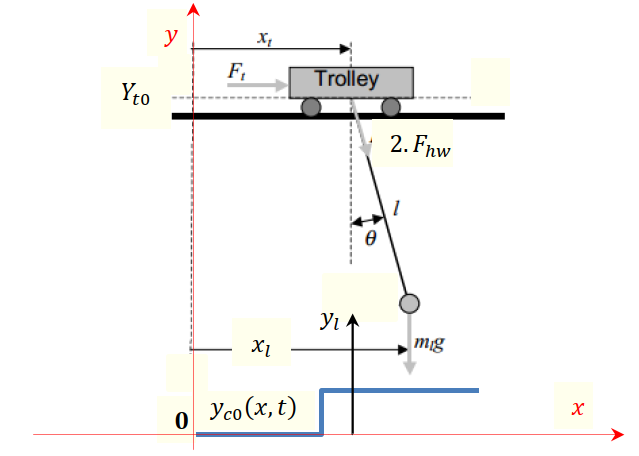
\includegraphics[width=0.5\textwidth]{figs/figure3_enunciado.png}
                \caption{Modelo físico simplificado del subsistema Carro – Cable – Carga y Perfil de Obstáculos}
                \label{fig:pendulo}
            \end{figure}
            
            \begin{equation}\label{eq:kinetic1}
                K = K_t + K_{lx} + K_{ly}
            \end{equation}
            \begin{equation}\label{eq:xl}
                x_l=x_t+l\sin{\theta}
            \end{equation}
            \begin{equation}\label{eq:dxl}
                \dot{x_l}=\dot{x_t}+l\cos{\theta}\dot{\theta}
            \end{equation}
            \begin{equation}\label{eq:y}
                y_l=Y_{t0}-l\cos{\theta}
            \end{equation}
            \begin{equation}\label{eq:dy}
                \dot{y_l}=-l\sin{\theta}\dot{\theta}
            \end{equation}

            \begin{equation}\label{eq:kinetic2}
                K = \frac{1}{2}m_t\dot{x_t}^2   +\frac{1}{2}m_l\dot{x_l}^2  +\frac{1}{2}m_l\dot{y_l}^2
            \end{equation}

            \begin{equation}\label{eq:kinetic3}
                K = \frac{1}{2}m_t\dot{x_t}^2   +\frac{1}{2}m_l(\dot{x_t}+l\cos{\theta}\dot{\theta})^2  +\frac{1}{2}m_l(-l\sin{\theta}\dot{\theta})^2
            \end{equation}

            \begin{equation}\label{eq:kinetic4}
                    K = \frac{1}{2}m_t\dot{x_t}^2 +\frac{1}{2}m_l(\dot{x_t}^2+l^2\cos^2{\theta}\dot{\theta}^2
                    +2l\dot{x_t}\cos{\theta}\dot{\theta})+\frac{1}{2}m_ll^2\sin^2{\theta}\dot{\theta}^2
            \end{equation}

            \begin{equation}\label{eq:potential}
                U = -m_lgl\cos{\theta}
            \end{equation}
            \begin{equation}\label{eq:lagrange}
                L = K - U
            \end{equation}

            \begin{equation}\label{eq:lagrange2}
                    L = \frac{1}{2}m_t\dot{x_t}^2
                    +\frac{1}{2}m_l(\dot{x_t}^2
                +l^2\cos^2{\theta}\dot{\theta}^2
                +2l\dot{x_t}\cos{\theta}\dot{\theta})
                +\frac{1}{2}m_ll^2\sin^2{\theta}\dot{\theta}^2
                +m_lgl\cos{\theta}
            \end{equation}

            \begin{equation}\label{eq:lagrange3}
                L = \frac{1}{2}m_t\dot{x_t}^2+\frac{1}{2}m_l\dot{x_t}^2
                +\frac{1}{2}m_ll^2\dot{\theta}^2
                +m_l\dot{x_t}l\cos{\theta}\dot{\theta}
                +m_lgl\cos{\theta}
            \end{equation}

            Se define el sistema de ecuaciones de Euler-Lagrange:
            \begin{equation}\label{eq:euler1}
                \frac{d}{dt}\left(\frac{\partial L}{\partial \dot{q}_i}\right)-\frac{\partial L}{\partial q_i}=Q_i
            \end{equation}

            Para \(q_i = x_t\):
            \begin{equation}\label{eq:euler2}
                \frac{d}{dt}\left(\frac{\partial L}{\partial \dot{x}_t}\right)-\frac{\partial L}{\partial x_t}=Q_t
            \end{equation}
            \begin{equation}
                \frac{\partial L}{\partial \dot{x}_t}= (m_t+m_l)\dot{x}_t+m_ll\cos{\theta}\dot{\theta}
            \end{equation}
            \begin{equation}            
                    \frac{d}{dt}\left(\frac{\partial L}{\partial \dot{x}_t}\right)= 
                    (m_t+m_l)\ddot{x}_t+m_l l\cos{\theta}\ddot{\theta}-m_ll\sin{\theta}\dot{\theta}^2
            \end{equation}
            \begin{equation}
                \frac{\partial L}{\partial x_t}=0
            \end{equation}
            Entonces:
            \begin{equation}
                (m_t+m_l)\ddot{x}_t+m_l l\cos{\theta}\ddot{\theta}-m_l l\sin{\theta}\dot{\theta}^2=F_t(t)-b_{eqt} \dot{x}_t
            \end{equation}

            Para \(q_i = \theta\):

            \begin{equation}\label{eq:euler3}
                \frac{d}{dt}\left(\frac{\partial L}{\partial \dot{\theta}}\right)-\frac{\partial L}{\partial \theta}=Q_{\theta}
            \end{equation}

            \begin{equation}
                \frac{\partial L}{\partial \dot{\theta}}=m_l\dot{x_t}l\cos{\theta}+m_ll^2\dot{\theta}
            \end{equation}

            \begin{equation}
                    \frac{d}{dt}\left(\frac{\partial L}{\partial \dot{\theta}}\right)= m_l\ddot{x_t}l\cos{\theta} -m_l\dot{x_t}l\sin{\theta}\dot{\theta}+m_ll^2\ddot{\theta}
            \end{equation}

            \begin{equation}
                \frac{\partial L}{\partial \theta}=-m_l\dot{x_t}l\sin{\theta}\dot{\theta}-m_lgl\sin{\theta}
            \end{equation}

            Entonces:
            \begin{equation}
                m_l\ddot{x_t}l\cos{\theta} -m_l\dot{x_t}l\sin{\theta}\dot{\theta}+m_ll^2\ddot{\theta}+m_l\dot{x_t}l\sin{\theta}\dot{\theta}+m_lgl\sin{\theta}=0
            \end{equation}

            Finalmente, el sistema de ecuaciones que define el modelo del sistema carro-pendulo es:
            \begin{equation}
                \begin{cases}
                    (m_t+m_l)\ddot{x}_t+m_ll\cos{\theta}\ddot{\theta}-m_ll\sin{\theta}\dot{\theta}^2=F_t(t)-b_{eqt} \dot{x}_t\\
                    m_l\ddot{x_t}l\cos{\theta} -m_l\dot{x_t}l\sin{\theta}\dot{\theta}+m_ll^2\ddot{\theta}+m_l\dot{x_t}l\sin{\theta}\dot{\theta}+m_lgl\sin{\theta}=0
                \end{cases}
            \end{equation}

            \begin{empheq}[box=\fbox]{equation}
                \begin{cases}
                    (m_t+m_l)\ddot{x}_t + m_l l \cos{\theta} \ddot{\theta} - m_l l \sin{\theta} \dot{\theta}^2 = 0 \\
                    \ddot{x}_t \cos{\theta} + l \ddot{\theta} + g \sin{\theta} = 0
                \end{cases}
            \end{empheq}


            Para representar lo en el espacio de estados se definen las siguientes variables de estado \(x\) y entradas \(u\):
            \begin{equation}
                x = \begin{bmatrix}
                    \theta \\
                    \dot{\theta}
                \end{bmatrix}
            \end{equation}
            \begin{equation}
                u = \ddot{x_l}
            \end{equation}

            Entonces, se obtiene el siguiente modelo en el espacio de estados no lineal:

            \begin{equation}
                \begin{cases}
                    \dot{x} = f(x,u,t) ; x(0) = x_0 \\
                    y = h(x,u,t)
                \end{cases}
            \end{equation}

            donde:
            \begin{equation}
                f(x,u,t) = \begin{bmatrix}
                    \dot{\theta} \\
                    - \frac{(m_t+m_l)\ddot{x}_t}{m_l l \cos{\theta}} + \tan{\theta} \dot{\theta}^2
                \end{bmatrix}
            \end{equation}
            \begin{equation}
                h(x,u,t) = -\frac{l \ddot{\theta}}{\cos{\theta}}  - g \tan{\theta}
            \end{equation}

            Realizando la linealización del sistema en el punto de equilibrio \(\theta = \theta^*\), \(\dot{\theta} = \dot{\theta}^*\) y \(\ddot{x}_t = \ddot{x}_t^*\) se obtiene el siguiente modelo linealizado:

            \begin{equation}
                \begin{cases}
                    \dot{z} = Az + Bu \\
                    y = Cz + Dv
                \end{cases}
            \end{equation}

            Donde \(z = x - x^*\), \(u = \ddot{x}_t - \ddot{x}_t^*\), \(y = \theta - \theta^*\) y \(v = \dot{\theta} - \dot{\theta}^*\).

            \begin{equation}
                A = \begin{bmatrix}
                    0 & 1 \\
                    -\frac{(m_t+m_l)\ddot{x}_t\tan{\theta}}{m_l l \cos{\theta}} + \frac{\dot{\theta}^2}{\cos^2{\theta}} & 2 \tan{\theta} \dot{\theta}
                \end{bmatrix}
            \end{equation}

            \begin{equation}
                B = \begin{bmatrix}
                    0 \\
                     -\frac{1}{m_l l \cos{\theta}}
                \end{bmatrix}
            \end{equation}







       
        \subsubsection{Control de balanceo}
            \begin{equation}
                U=\ddot{X}_t= \left(k_d s+k_p\right) \frac{1}{s} \left(\dot{\Theta}^*- \dot{\Theta}\right)
            \end{equation}

            \begin{equation}
                U=\ddot{X}_t= \left(k_d +\frac{k_p}{s}\right) \left(\dot{\Theta}^*- \dot{\Theta}\right)
            \end{equation}
            
            \begin{equation}
                 s^2 \Theta = A_{21} \Theta + B_{2} \left(k_d +\frac{k_p}{s}\right) \left(\dot{\Theta}^*- \dot{\Theta}\right)
            \end{equation}

            \begin{equation}
                s \dot{\Theta} = A_{21} \frac{\dot{\Theta}}{s} + B_{2} k_d \dot{\Theta}^* - B_{2} k_d \dot{\Theta}  + B_{2} k_p \frac{\dot{\Theta}^*}{s}  - B_{2} k_p \frac{\dot{\Theta}}{s} 
            \end{equation}

            \begin{equation}
                s^2 \dot{\Theta} = A_{21} \dot{\Theta} + s B_{2} k_d \dot{\Theta}^* - s B_{2} k_d \dot{\Theta}  + B_{2} k_p \dot{\Theta}^* - B_{2} k_p \dot{\Theta}
            \end{equation}

            \begin{equation}
                \dot{\Theta}(s^2 - A_{21} + s B_{2} k_d + B_{2} k_p) = \dot{\Theta}^*(s B_{2} k_d + B_{2} k_p)
            \end{equation}

            \begin{equation}
                G(s)=\frac{\dot{\Theta}}{\dot{\Theta}^*}=\frac{s B_{2} k_d + B_{2} k_p}{s^2 + s B_{2} k_d + B_{2} k_p - A_{21}}
            \end{equation}

            \begin{equation}
                p_r(s)=(s^2+2\zeta\omega_n s+\omega_n^2)
            \end{equation}

            \begin{equation}
                \begin{cases}
                    \omega_n^2 = B_{2} k_p - A_{21}\\
                    2\zeta\omega_n = B_{2} k_d
                \end{cases}
            \end{equation}

            \begin{equation}
                \begin{cases}
                    k_p = \frac{\omega_n^2 + A_{21}}{B_{2}}\\
                    k_d = \frac{2\zeta\omega_n}{B_{2}}
                \end{cases}
            \end{equation}

        \subsection{Generación de trayectorias}

            La generación de trayectorias se implementa cuando la grúa opera en modo automático. Su función es definir un perfil que posicione a la grúa en una ubicación \textit{xy} determinada de manera suave y eficiente. Para ello, se genera una matriz que describe la posición, velocidad y aceleración de cada motor en función del tiempo, utilizando un intervalo de tiempo \textit{dt}. La trayectoria considera la posición actual de la grúa y la columna de contenedores o bahía de carga de destino. Además, se tiene en cuenta el perfil de obstáculos y se establece una distancia de seguridad en las direcciones \textit{x} e \textit{y}, definiendo así una zona de seguridad en la que el modo automático no puede operar.

            En primer lugar, se definen los puntos significativos de la trayectoria: la posición inicial, la posición final y la altura máxima. Estos puntos se calculan considerando el perfil de obstáculos previamente mencionado.

            Posteriormente, se calculan los perfiles de subida, bajada y traslación. Estos perfiles se ajustan teniendo en cuenta los estados inicial y final deseados, asegurando así que el movimiento sea suave. Los perfiles se determinan utilizando un perfil de aceleración trapezoidal, que incluye una sobreaceleración para lograr una trayectoria más fluida y eficiente. La figura \ref{fig:perfil} ilustra un ejemplo de un perfil de aceleración trapezoidal similar al que se utiliza. Se indican siete tiempos que definen el perfil necesario para alcanzar un estado deseado. En este perfil, se observa que tanto la velocidad como la aceleración inicial son distintas de cero, y el perfil se ajusta a estos valores de manera que la transición entre el estado inicial y el perfil sea suave.

            \begin{figure}[H]
                \centering
                \includegraphics[width=1\textwidth]{figs/Figure_trap_profile.png}
                \caption{Perfil de aceleración trapezoidal con condiciones iniciales \(x_0=0 \, \text{m}\), \(v_0=1 \, \text{m/s}\) y \(a_0=-1.5 \, \text{m/s}^2\).}
                \label{fig:perfil}
            \end{figure}

            Es importante destacar que la generación de la trayectoria admite casos degenerados, lo que contribuye a la robustez del sistema. Se aceptan situaciones en las que la distancia recorrida es menor que la requerida para alcanzar la aceleración o velocidad máxima. En estos casos, se ajustan los perfiles utilizando un algoritmo recursivo para adaptar el perfil trapezoidal a uno triangular, como se muestra en la figura \ref{fig:perfilTriangular}.

            \begin{figure}[H]
                \centering
                \includegraphics[width=1\textwidth]{figs/Figure_trap_profile_triangle.png}
                \caption{Perfil de aceleración en un caso degenerado.}
                \label{fig:perfilTriangular}
            \end{figure}

            Con los cálculos de estos perfiles, se realiza un análisis del tiempo que toma cada uno de los movimientos. En función de estos tiempos y del perfil de obstáculos, se determina un solapamiento en los movimientos, de modo que la grúa no se detenga en ningún momento, acortando así los tiempos de translación. La figura \ref{fig:trayectoria} muestra un ejemplo de la trayectoria junto con el perfil de obstáculos.

            \begin{figure}[H]
                \centering
                \includegraphics[width=0.8\textwidth]{figs/Figure_trayectoria.png}
                \caption{Trayectoria de la carga.}
                \label{fig:trayectoria}
            \end{figure}

            La sincronización del movimiento y la suavidad del desplazamiento se pueden corroborar en las figuras \ref{fig:posicion_carro_izaje} y \ref{fig:velocidad_carro_izaje}.

            \begin{figure}[H]
                \centering
                \includegraphics[width=0.8\textwidth]{figs/Figure_posicion_carro_izaje.png}
                \caption{Posición del carro e izaje.}
                \label{fig:posicion_carro_izaje}
            \end{figure}

            \begin{figure}[H]
                \centering
                \includegraphics[width=0.8\textwidth]{figs/Figure_velocidad_carro_izaje.png}
                \caption{Velocidad del carro e izaje.}
                \label{fig:velocidad_carro_izaje}
            \end{figure}




\section{Resultados}\label{sec:results}

\section{Conclusión}\label{sec:conclusion}


% Estilo de citas
%\bibliographystyle{unsrt}

% Nombre del archivo .bib
%\bibliography{references}

\end{document}